% arXiv-friendly version of the paper
\documentclass[12 pt]{amsart}

\usepackage{amsmath}
\usepackage{amssymb}
\usepackage{amsfonts}

\usepackage[largesc]{newpxtext}
\usepackage[varbb]{newpxmath}
\usepackage{float}

% wider margins just for now, so that todonotes are easily visible
\usepackage[margin = 1.5 in]{geometry}
\usepackage{microtype}
\usepackage[indent]{parskip}

% theorem setup
\usepackage{amsthm, thmtools, thm-restate}
\newtheorem{theorem}{Theorem}[section]
\newtheorem{proposition}[theorem]{Proposition}
\newtheorem{corollary}[theorem]{Corollary}
\newtheorem{lemma}[theorem]{Lemma}
\newtheorem{conjecture}[theorem]{Conjecture}
\theoremstyle{definition} % definition style
\newtheorem{definition}[theorem]{Definition}
\newtheorem{example}[theorem]{Example}
\theoremstyle{remark} % remark style
\newtheorem{remark}[theorem]{Remark}

\usepackage{hyperref, cleveref}
\hypersetup{ % make links pretty and not boxed
colorlinks,
linkcolor = blue,
urlcolor = blue,
citecolor = blue}

% car
\newcommand{\mzncar}[3][(0,0)]{
\begin{scope}[shift={#1}]
\shade[top color=#2, bottom color=#3, shading angle=90, draw=white, rounded corners=0.7ex, very thick] (0.75,.25) -- ++(0,0.5) -- ++(0.5,0.15) -- ++(1.5,0) -- ++(0.5,0) -- ++(0,-0.65) -- (0.75,.25) -- cycle;
\draw[thick, rounded corners=0.2ex, fill=white, thick] (1.25,0.85) -- ++(0.5,0.35) -- ++(0.8,0) -- ++(0.3,-0.35) -- (1.25,0.85);
\draw[thick] (2.1,0.85) -- (2.1,1.2);
\draw[fill=gray!80,thin] (1.375,.25) circle[radius=.2];
\draw[fill=gray!80,thin] (2.76,.25) circle[radius=.2];
\end{scope}
}

% add your own todostyle!
\usepackage{todonotes}
\todostyle{jayden}{color = pink}
\todostyle{jasper}{color = lime}
\todostyle{alan}{color = purple}

\title{Preference-restricted parking functions}

\author[Bown]{Jasper Bown}
\address[J. Bown]{Harvey Mudd College, United States}
\email{abown@g.hmc.edu}

\author[Kagey]{Peter Kagey}
\address[P. Kagey]{California State Polytechnic University, Pomona}
\email{pkagey@cpp.edu}

\author[Kappler]{Alan Kappler}
\address[A. Kappler]{Harvey Mudd College, United States}
\email{akappler@g.hmc.edu}

\author[Orrison]{Michael E.~Orrison}
\address[M.~Orrison]{Harvey Mudd College, United States}
\email{orrison@hmc.edu}

\author[Thadani]{Jayden Thadani}
\address[J. Thadani]{Harvey Mudd College, United States}
\email{jthadani@hmc.edu}


\begin{document}
	

\begin{abstract}
	We demonstrate a new paradigm for solving parking problems --- preference-restricted parking functions. By considering parking functions on $n$ cars where all cars prefer spots in some convenient $S \subseteq [n]$, we convert questions about complicated parking procedures into more easily understood questions about ordinary parking functions. In particular, we demonstrate choices of $S$ that yield new combinatorial insights into previous results about variant parking procedures, distinct enumerations of ``parking functions'' for those parking procedures, a novel characterization of prime parking functions, and Abel's binomial theorem.
\end{abstract}

\maketitle

\pagebreak

\tableofcontents

\pagebreak

% just set up to make sure the todo list gets printed fine at the start of the doc
\makeatletter
\providecommand\@dotsep{5}
\makeatother
\listoftodos\relax

\pagebreak

\section{Introduction}

The classical parking function problem is to describe the parking preferences of cars that allow every car to park under a certain parking procedure. Each of $n$ cars goes down a one-way parking lot with $n$ parking spots, attempts to park in its preferred spot, and then each subsequent spot until it parks.

The \emph{parking functions} on $n$ cars are those $\pi : [n] \to [n]$ which take each of $n$ cars to their preferences in a manner that allows all cars to park, are well understood. \todo[jayden]{explain the Catalan condition} However, many variants of the parking function question considered in the literature do not fully leverage our understanding of parking functions ---
\begin{enumerate}
	\item What if there are fewer cars than spots? How can we minimize the number of cars unable to park? (A special case of the variants considered in \cite{cameron-johannsen-prellberg-schweitzer-2008}.)
	\item What if each parking spot can accommodate more than one car? (Perhaps, as in \cite{blake-konheim-1977}, our parking spots are hash buckets, and our cars are data.)
	\item Prime parking functions --- the building blocks from which parking functions are formed.
\end{enumerate}
We will show that all of these can be understood as \emph{$S$-restricted parking functions} --- parking functions $\pi : [n] \to S \subseteq [n]$.

\begin{definition}
    An $S$-restricted parking function on $n$ cars, given a set of possible preferences $S$ is a parking function $\pi$ on $n$ cars where all preferences lie in $S$ --- $\pi([n]) \subset S$.

    We denote the set of $S$-restricted parking functions by $\mathrm{PF}_{n \mid S}$ and thus, their number by $\# \mathrm{PF}_{n \mid S}$.
\end{definition}


These reinterpretations yield new combinatorial insights, simpler proofs, and connections to deep results in combinatorics. In some sense, $S$-restricted parking functions is a paradigm for solving parking questions that strikes the balance between the generality of $\mathbf{u}$-parking functions --- of which they are the special case $\mathbf{u} = ( \# [1] \cap S , \dots, \# [n] \cap S)$ \todo[jayden]{use absolute value symbol} --- and the obvious combinatorial intuition of the original parking function question.

\section{Initial segment restrictions} \todo[jayden]{swap this and prime parking functions}

%$S$-restricted parking functions are closely related to a certain class of vector (or $\mathbf{u}$-)parking functions, associated to vectors $\mathbf{u}=(u_1,u_2,u_3,\ldots,u_n)$ and defined by \cite{} as preference functions whose $i$th-smallest preference is at most $u_i.$

%\begin{theorem}
%    For any $S\subseteq[n],$ $S$-restricted parking functions are in bijection with the $\mathbf{u}$-parking functions associated to $u_i=|S\cap [i]|.$
%\end{theorem}

%\begin{proof}
%    Letting $s=|S|,$ take the function $f:[s]\to S$ given by 
%\end{proof} \todo[jayden]{I think this could be just a short note in the introduction after the ``balance between the power of $\mathbf{u}$-parking functions'' comment --- I'm not sure we need a proof}

Note that since every parking function has at least one preference equal to $1,$ $\# \mathrm{PF}_{n\mid S}$ is only nonzero when $1\in S.$ One natural type of restriction to look at, then, is one where only the first few spots can be preferred. Specifically, we look at restrictions to $[s],$ where $1\le s\le n.$

This type of set is closely related to another variant on classical parking functions, when the number of cars differs from the number of spots to park in. \cite{cameron-johannsen-prellberg-schweitzer-2008} studies this idea in some depth. One particularly interesting case occurs when there are more cars than parking spots; not all cars will be able to park, but we can try to minimize the defect of the system (that is, the number of cars which are unable to park).

\begin{theorem}
    Given $1\le s\le n,$ the number of ways for $n$ cars to park in $s$ spots, with the minimum possible defect of $n-s,$ is equal to $\# \mathrm{PF}_{n \mid [s]}.$
\end{theorem}

\begin{proof}
    We have in both situations a set of preference functions on $n$ cars and taking values in $[s]$; we'd like to prove that they coincide. To do so, add to the end of our street of $s$ spots an extra segment of length $n-s$ that catches the overflow. Our case with minimum defect will occur only when the overflow segment is exactly full: that is, if all cars can park in one of the $s+(n-s)=n$ spots we've constructed.

    But this is exactly analogous to our parking procedure! We have $n$ cars parking in the first $s$ of $n$ spots, and a parking function only occurs when all cars can park. We are counting the same procedure in two different ways --- thus the equality.
\end{proof}

One question we can ask: how many $[s]$-restricted parking functions are there? This is answered by \cite{cameron-johannsen-prellberg-schweitzer-2008} through a combinatorial proof, reproduced here in the language of $[s]$-restricted parking functions:

\begin{restatable}{theorem}{resPFcount1}
    \label{thm:resPFcount1}
    Let $1\le s\le n.$ Then the number of $[s]$-restricted parking functions on $n$ cars is
    \[s^{n} - \sum_{i = 0}^{s - 1} \binom{n}{i} (i + 1)^{i - 1} (s - i - 1)^{n - i}.\]
\end{restatable}

\begin{proof}
    There are $s^{n}$ possible preference lists in $[s]^{n}$, when not considering the constraint of being a parking function. If $\pi \in [s]^{n}$ is not a parking function, then there must be an unoccupied spot somewhere among the $n$ spots; all such unoccupied spots lie in $[s],$ since least $n - s$ cars come to the last $c - s$ spots by the minimum-defect argument above, filling all spots except for (potentially) the first $s$.

	Let $i$ be the number of spots before the first unoccupied spot. Then there must be $i$ cars that form a parking function on those first $i$ spots. Choose those $i$ cars in one of $\binom{n}{i}$ ways, and one of the $(i + 1)^{i - 1}$ parking functions of length $i$. None of the remaining $n - i$ cars can prefer any of the first $i + 1$ spots; otherwise at least $i+1$ cars have preferences in the first $i+1$ spots, so at least one of them will be forced to proceed to spot $i+1$. However, they all can prefer any of the remaining $s - i - 1$ spots in one of $(s - i - 1)^{n - i}$ ways. This makes for $\binom{n}{i} (i + 1)^{i - 1}(s - i - 1)^{n - i}$ preference lists in $[s]^{n}$ so that the first unoccupied spot is $i + 1$. Subtracting the sum over all possible $i$ from the number of total preference lists gives
	\[
		\# \mathrm{PF}_{n \mid [s]} = s^{n} - \sum_{i = 0}^{s - 1} \binom{n}{i} (i + 1)^{i - 1} (s - i - 1)^{n - i},
	\]
    as desired.
\end{proof}

This expression is one half of a sum given by Abel's binomial theorem, as noted by \cite{cameron-johannsen-prellberg-schweitzer-2008} and expanded upon below. We present a combinatorial proof corresponding to the other half of that sum, which (as far as we can tell) is novel:

\begin{restatable}{theorem}{resPFcount2}
    \label{thm:resPFcount2}
    The number of $[s]$-restricted parking functions on $n$ cars may be expressed as
    \[\sum_{i = s}^{n} \binom{n}{i} (i + 1)^{i - 1} (s - i - 1)^{n - i}.\]
\end{restatable}

\begin{proof}
    Our goal here will be to take all parking functions on $n$ cars and eliminate those with cars that prefer spots in $[n] \setminus [s]$. We do so by means of an alternating sum that counts every parking function positively and negatively an equal number of times, \textit{unless} its preferences lie entirely within $[s].$

	We consider 2-colored parking functions --- that is, parking functions with cars assigned one of two colors --- with a particular restriction upon them.  Suppose we choose a subset of size $i \ge s$ of our cars to be colored indigo. These cars are to form a parking function on the first $i$ parking spots (though the parking outcome may not result in them actually parking there). The remaining $n - i$ cars are colored red and can prefer any of the $i + 1 - s$ ``forbidden'' spots in  $[i + 1] \setminus [s]$.
    
\begin{figure}
\begin{center}
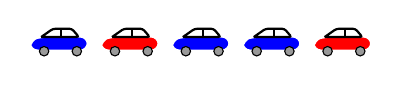
\begin{tikzpicture}[scale=0.3]
	\mzncar[(0,0)]{blue}{blue} \mzncar[(3,0)]{red}{red} \mzncar[(6,0)]{blue}{blue} \mzncar[(9,0)]{blue}{blue} \mzncar[(12,0)]{red}{red}
\end{tikzpicture} $\quad \longleftrightarrow \quad$
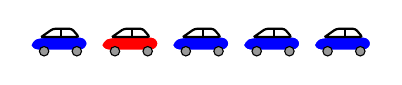
\begin{tikzpicture}[scale=0.3]
	\mzncar[(18,0)]{blue}{blue} \mzncar[(21,0)]{red}{red} \mzncar[(24,0)]{blue}{blue} \mzncar[(27,0)]{blue}{blue} \mzncar[(30,0)]{blue}{blue}
\end{tikzpicture}
\end{center}
\caption{For $n=5$, $s = 2$, two colorings of $\pi = (1,3,2,2,4)$ with $i = 3$ and $i = 4$ are connected by recoloring car 5. Note that both satisfy the constraints of the proof below.}
\end{figure}
    
    These preferences always form a parking function --- the Catalan condition is satisfied up to spot $i$ by the indigo cars since they form a parking function, and then the red cars all prefer one of the first $i + 1$ spots, satisfying the condition from $i+1$ onwards.
    
    We count these parking functions positively when there are an even number of red cars and negatively otherwise. This count is
	\[
		\sum_{i = s}^{n} \binom{c}{i} (i + 1)^{i - 1} (i + 1 - s)^{c - i} (-1)^{c - i}.
	\]
	This is equal to the sum above; note that consecutive terms have opposite sign.

	We now create a sign-reversing involution on these 2-colored parking functions (Figure 1). If $m$ is the maximum preference among all the cars, let car $x$ be the first car that prefers spot $m$ (this choice is arbitrary, but one such car must be specified). That is, for a parking function $\pi$, let \[x = \min(\pi^{-1}(m)),\] where $m=\max(\pi([n]))$. Note that $m > s$ as long as there exist any red cars, since red cars all prefer spots greater than $s$. For our involution, we recolor this car, making it red if it was indigo and vice versa. 

	If car $x$ was red, then  $m\in [i + 1]$ by definition. Consider the same parking function with car $x$ painted indigo. Adding any preference in $[i + 1]$ to a parking function of length $i$ will form a parking function of length $i + 1$. To see this, consider adding the preference at the end. The first $i$ cars will park in the first $i$ spots (on which they form a parking function), and then the added car will park in the last spot. Since parking functions are permutation invariant, the list will form a parking function no matter where we add the car. Thus, with car $x$, the indigo cars form a parking function of length $i + 1$.
    
    Since the red cars with car $x$ formed a subset of $[i + 1] \setminus [s]$, without car $x$ they certainly form a subset of the larger $[i + 2] \setminus [s]$. Both conditions are thus satisfied for one direction of the involution.

	If car $x$ was indigo, then $m \in [i]$ (since the $i$ indigo cars form a parking function). Consider the same parking function with car $x$ painted red. The remaining indigo cars will still form a parking function on $i - 1$ cars: the $j$th smallest preference will still be at most $j$ after removing the maximum preference, so the Catalan condition is still satisfied.
    
    Since $m \in [i]$ was the maximum preference, all red cars' preferences will be in $[i].$ No old red cars will be in $[s],$ since all were contained in $[i+1]\backslash [s]$ The new red car is the only thing to worry about: all red cars will have preferences in $[i]\backslash [s],$ and therefore all conditions will be satisfied for the involution, unless $m\in [s].$

	This is our exception --- we cannot recolor to have a new red car if even the maximum preference is in $[s]$. This corresponds to the the $[s]$-restricted parking functions of length $c$. They are only counted once --- positively, as a subset of the term with 0 red cars. Any other pair of 2-colored parking functions is counted positively once and negatively once in our sum, for an even and odd number of red cars respectively. Thus, the sum counts only $\#\mathrm{PF}_{c \mid [s]}$.
\end{proof}

There is an analogous result for prime parking functions as well! Recall that these are preference functions $\pi:[n]\to[n]$ that satisfy an extra-strong Catalan condition, that at least $i$ cars have preferences in $[i-1]$ for all $1<i\le n.$ These are a subset of all parking functions, and their total count is $(n-1)^{n-1}$. They are discussed further in \cref{primesection}. This motivates the following definition:

\begin{definition}
    An $S$-restricted prime parking function on $n$ cars, is a parking function on $n$ cars where all preferences lie in $S.$ We denote the number of parking functions of this type as $\# \mathrm{PPF}_{n\mid S}.$
\end{definition}

We can enumerate restrictions on prime parking functions in much the same manner as we did normal parking functions:

\begin{theorem}
    \label{thm:resPPFcount1}
    For $1 \le s < n,$ the number of $[s]$-restricted parking functions on $n$ cars which are also prime is 
    \[s^{n} - (s - 1)^{n} - \sum_{i = 1}^{s} \binom{n}{i} (i - 1)^{i - 1} (s - i)^{n - i}.\]
\end{theorem}

\begin{proof}
	Our goal is again to take all $s^n$ restricted preference functions and remove those which are not prime parking functions. A prime parking function must have its 1st, 2nd, 3rd, 4th, etc. smallest preferences be at most $1,1,2,3,\ldots$; we do casework on the first counterexample. We treat the first case separately: there are $(s-1)^n$ ways to have one's smallest preference greater than 1, as we must choose preferences from $2$ to $s$ for each car.
    
    Now we can assume that some $i\in [s-1]$ is the smallest value such that the $i+1$th value is greater than $i$. Since more than $j$ cars prefer the first $j$ spots for all $j < i+1$, the $i$ cars that prefer the first $i$ spots form a prime parking function on $[i]$ in one of $(i - 1)^{i - 1}$ ways. The remaining $n - i$ cars can prefer any of the remaining $s - i$ spots in $[s] \setminus [i]$ in one of $(s - i)^{n - i}$ ways. With $\binom{c}{i}$ ways to choose the $i$ cars, there are $\binom{n}{i} (i - 1)^{i - 1} (s - i)^{n - i}$ preference lists in $[s]^{n}$ so that the first counterexample is $i+1$.

    This means that subtracting off all possible non-prime parking functions gives
	\[
		\# \mathrm{PPF}_{n \mid [s]} = s^{n} - (s - 1)^{n} - \sum_{i = 1}^{s} \binom{n}{i} (i - 1)^{i - 1} (s - i)^{n - i}
	\]
    as desired.
\end{proof}

\begin{theorem}
    \label{thm:resPPFcount2}
    For $1 \le s < n,$ the number of $[s]$-restricted parking functions on $n$ cars which are also prime may be expressed as
    \[\sum_{i = s + 1}^{n} \binom{n}{i} (i - 1)^{i - 1} (s - i)^{n - i}\]
\end{theorem}

\begin{proof}
    We proceed similarly to \cref{thm:resPFcount2}, with modifications to account for prime parking functions.
    
    We will now count 2-colored prime parking functions. The $i$ indigo cars are to form a prime parking function on $[i]$; the remaining $n - i$ cars are colored red and can prefer any of the $i - s$ forbidden spots in  $[i] \setminus [s]$. These preferences always form a prime parking function --- the extra-strong Catalan condition is satisfied up to spot $i-1$ by the indigo cars since they form a prime parking function, and then the red cars all prefer one of the first $i$ spots, satisfying the condition from $i$ onwards. We count these parking functions positively with an even number of red cars and negatively otherwise. This count is
	\[
		\sum_{i = s}^{c} \binom{c}{i} (i - 1)^{i - 1} (i - s)^{c - i} (-1)^{c - i},
	\]
	equal to the sum above.

	We use the same involution as before: recolor car $x,$ the first car that has the maximum preference $m.$ Note that $m > s$ as long as there are some red cars, since the red cars all prefer spots greater than $s$.

	If car $x$ is painted red, then  $m \in [i]$ just by definition. We can reconstruct the same parking function with car $x$ painted indigo. We can add any preference in $[i]$ to a prime parking function of length $i$ and the list will form a prime parking function of length $i + 1,$ by the same argument as above.
    
    Since the red cars with car $x$ formed a subset of $[i] \setminus [s]$, without car $x$ they also form a subset of the larger $[i + 1] \setminus [s]$. Thus all conditions are satisfied and our involution works in one direction.

	If car $x$ is painted indigo, then $m\in [i-1]$ for the indigo cars to form a parking function. Thus, we can reconstruct the same parking function with car $x$ repainted red. The remaining indigo cars will still form a prime parking function on $i - 1$ cars --- the $j$th smallest preference will still be less than $j$ after removing the maximum preference.
    
    Since $m\in [i-1]$ was the maximum preference, all red cars will be in $[i-1]$. No old red cars will be in $[s],$ since all were contained in $[i]\backslash [s].$ The new red car is the only thing to worry about: all red cars will have preferences in $[i-1]\backslash [s],$ and therefore all conditions will be satisfied for the involution, unless $m\in [s].$

	Once again, then, we have a single exception to the involution: prime parking functions where all preferences are in $[s]$ are counted once while everything else cancels. Thus our alternating sum counts $\mathrm{PPF}_{c \mid [s]}$.
\end{proof}

\subsection*{Abel's binomial theorem}

In enumerating $[s]$-restricted parking functions and their prime variants, we demonstrated two different counts for each --- one by excluding all of the restricted preference lists that aren't the desired type of parking function, another by taking all parking functions and allowing those with forbidden preferences to cancel. The expressions we get from these two approaches are very similar; this isn't a coincidence!

Abel's binomial theorem is a generalization of the standard binomial theorem, with deep roots in the theory of reluctant functions and forests. The identity has many equivalent statements. One common form similar to those in \cite{shapiro-1991} and \cite{zucker-2024} is that
\[
	(X + Y)^{n} = \sum_{i = 0}^{n} \binom{n}{i} X (X + iZ)^{i - 1} (Y - i Z)^{n - i}.
\]
for $X, Y, Z \in \mathbb{C}$ and $n \in \mathbb{Z}_{> 0}$. The substitutions $x = X/Z$ and $y = Y/Z - n$ (for suitable $Z$) yield an equivalent form that is particularly amenable to combinatorial interpretation --- our enumerations of $[s]$-restricted parking functions are really two different truncations of the identity.

\begin{restatable}[Abel's binomial theorem]{theorem}{abelsbin}
	For all $n\in\mathbb{Z}_{>0}$ and $x,y\in\mathbb{C},$
    \[
		(x + y + n)^{n} = \sum_{i = 0}^{n} \binom{n}{i} x (x + i)^{i - 1} (y + n - i)^{n - i}.
	\]
\end{restatable}

Since the expressions in \cref{thm:resPFcount1} and \cref{thm:resPFcount2} both count $[s]$-restricted parking functions on $n$ cars, we can set them equal. With all the sums on one side, we see
\begin{align*}
    s^{n} &= \sum_{i = 0}^{s - 1} \binom{n}{i} (i + 1)^{i - 1} (s - i - 1)^{n - i} + \sum_{i = s}^{n} \binom{n}{i} (i + 1)^{i - 1} (s - i - 1)^{n - i}\\
    &=\sum_{i = 0}^{n} \binom{n}{i} (i + 1)^{i - 1} (s - i - 1)^{n - i},
\end{align*}
which is Abel's theorem for $x=1,$ $y=s-n-1.$ Similarly, from \cref{thm:resPPFcount1} and \cref{thm:resPPFcount2} we get 
\begin{align*}
    - (s - 1)^{n} &= -s^n + \sum_{i = 1}^{s} \binom{n}{i} (i - 1)^{i - 1} (s - i)^{n - i} + \sum_{i = s + 1}^{n} \binom{n}{i} (i - 1)^{i - 1} (s - i)^{n - i}\\
    &=\sum_{i=0}^n \binom{n}{i} (i - 1)^{i - 1} (s - i)^{n - i},
\end{align*}
which is Abel's theorem for $x=-1,$ $y=s-n+1$. It's rather surprising that we'd find this-- there's no clear reason why these two sums should merge, especially considering that one half of the sum is alternating and the other isn't!

These are merely special cases, but we can actually recover the complete form of the identity from this! To do so, we'll need a result from \cite{yan-survey-2015}, giving a generating function for the number of preferences for the first spot in a parking function: %\todo[jayden]{apparently there's also a Pollak-style argument for this (Stanley hints at it in some slides that I can't find)}

\begin{lemma}
    The sum over all length-$n$ parking functions $\pi$ of $x^{|\pi^{-1}(\{1\})|}$ is $x(x+n)^{n-1}$ for any $n\in\mathbb{Z}_{>0}.$
\end{lemma}

Note that this reduces to the usual $(n+1)^{n-1}$ when setting $x=1$; Yan uses a clever construction involving a bijection with labeled trees. This gives us a rather more general form for our identity:

\begin{theorem}
    \label{thm:res-1s-enumerator}
    The sum over $[s]$-restricted length-$n$ parking functions $\pi$ of $x^{|\pi^{-1}(\{1\})|}$ may be expressed as
    \[(s-1+x)^{n} - \sum_{i = 0}^{s - 1} \binom{n}{i} x(x + i)^{i - 1} (s - i - 1)^{n - i},\]
    or as
    \[\sum_{i = s}^{n} \binom{n}{i} x(x + i)^{i - 1} (s - i - 1)^{n - i}.\]
\end{theorem}

\begin{proof}
    We omit most of the details here, as they follow along lines very similar to \cref{thm:resPFcount1} and \cref{thm:resPFcount2}.
    
    For the first claim, $(s-1+x)^n$ is a generating function for all preference functions restricted to $[s],$ as the number of preference functions with $k$ 1s is $\binom{n}{k}1^k(s-1)^{n-k}.$ In each term of the sum we're subtracting off, $x(x+i)^{i-1}$  counts parking functions of length $i$; the $(s-i-1)^{n-i}$ represents preferences after the first gap in the parking lot, and therefore it has no 1s to account for.

    The second claim proceeds similarly; $x(x+i)^{i-1}$ again counts parking functions of length $i$. Since $(s-i-1)^{n-i}$ counts red cars, which always prefer forbidden spots greater than $s\ge1,$ we again needn't account for preferences of 1 here. From this point on the proofs are identical.
\end{proof}

\begin{proof}[Proof of Abel's binomial theorem]
	Equating the two expressions in the previous theorem gives us that for all $n\in\mathbb{Z}_{>0},$ $s\in [n],$ $x\in\mathbb{C},$
	\[
		(s-1+x)^{n} = \sum_{i = 0}^{n} \binom{n}{i} x(x + i)^{i - 1} (s - i - 1)^{n - i}.
	\]
In particular, viewing both sides of the expression as a polynomial in $s$: for any $n\in\mathbb{Z}_{>0}$ and $x\in\mathbb{C},$ we have two monic polynomials $f(s)$ and $g(s)$ of degree $n$ which agree on $n$ distinct values. These must then be equal, since $f(s)-g(s)$ is of degree at most $n-1$ and has at least $n$ roots --- $f(s) - g(s)$ is the zero polynomial.

Thus the above identity is true for all $x,s\in\mathbb{C}$ and $n\in\mathbb{Z}_{>0}$. Substituting $s=n+1+y$ recovers Abel's binomial theorem.

\end{proof}

\subsection*{The symmetric group and initial restrictions}

Regular parking functions (on $n$ cars) have certain structure beyond just whether they are parking functions or not. For example, whether a given $\pi : [n] \to [n]$ is a parking function depends only on the size of each of the pre-images $\pi^{-1}([i])$. It doesn't matter which cars prefer spots in each $[i]$. However, the parking function itself also comes with the data of its \emph{parking outcome} (the permutation sending each parking space to the car parked in it) which clearly does depend on which cars prefer spots. This structure involves the symmetric group $\mathfrak{S}_{n}$ in two different ways.

First, there is an action of the symmetric group on $\mathrm{PF}_{n}$ by shuffling around the preferred spots among the cars. Explicitly, this is the left action $\mathfrak{S}_{n} \times \mathrm{PF}_{n} \to \mathrm{PF}_{n}$ by $\sigma \cdot \pi = \pi \circ \sigma^{-1}$. Counting the orbits of this action is equivalent to counting the ``non-decreasing'' (order-preserving) parking functions. It's known that they are in bijection with Dyck paths and thus, the number of them is the $n$th Catalan number $C_{n}$ (see, for example, \cite{armstrong-loehr-warrington-2016}).

Second, there is a surjection $\mathrm{PF}_{n} \twoheadrightarrow \mathfrak{S}_{n}$ that sends every parking function to its parking outcome. Every parking outcome must be a bijection $[n] \to [n]$ from spots to cars --- a permutation; every permutation can be achieved by a parking function that is the same permutation. In \cite{pinsky-2024}, Pinsky determines the size of the pre-image of a permutation $\sigma \in \mathfrak{S}_{n}$ under this map, and analyses asymptotics as $n \to \infty$.

Both of these analyses have analogues for $[s]$-restricted parking functions. \todo[jayden]{prove them}

\begin{theorem}
	Under the described action of $\mathfrak{S}_{n}$ on $\mathrm{PF}_{n \mid [s]}$ there are $C(n, s - 1)$ orbits.

	Here $C(n, k)$ is the $(n, k)$th entry in Catalan's triangle, also known as the Narayana number $N(n, k)$ \cite[A001263]{oeis}.
\end{theorem} 

\begin{theorem}
    The number of $[s]$-restricted parking functions on $n$ cars with parking outcome $\sigma \in \mathfrak{S}_m$ is
    \[
    \prod_{i=1}^m \max(0,l_{m,i}(\sigma)-\max(0,i-n)).
    \]
    Here $l_{m, i}$ is the length of the longest contiguous string in $\sigma$ (written in one-line notation as $\sigma_{1} \cdots \sigma_{n}$) ending at $\sigma_i$ with $\sigma_i$ greater than any other $\sigma_{j}$ within the string.
\end{theorem}




\section{Prime parking functions} \label{primesection}

Prime parking functions are an important class of parking functions. In analogy with primes, they are the indecomposable parts from which all parking functions are built. They are often defined as satisfying a stricter condition than parking functions. See \cite{armon-2024} for a further discussion of these functions.

\begin{definition}[prime parking functions]
	A prime parking function on $n$ cars is a preference function $\pi : [n] \to [n]$ such that more than $i$ cars prefer the first $i$ spots (for $1 \le i \le n$). In other words $\# \pi^{-1}([i]) > i$.
\end{definition}

Prime parking functions themselves have a characterization in terms of $S$-restricted parking functions --- prime parking functions are in bijection with parking functions where no car prefers the second spot. Essentially, this bijection follows by reassigning cars' preferences in certain manner to turn a restricted parking function into a prime parking function.

\begin{restatable}{theorem}{primeIsRes}
    \label{thm:primeIsRes}
	There is a bijection between prime parking functions and $[n] \setminus \{ 2 \}$-restricted parking functions (on $n$ cars). That is,
	\[
		\# \mathrm{PPF}_{n} = \# \mathrm{PF}_{n \mid [n] \setminus \{ 2 \}} 
	\]
\end{restatable}

In fact, this generalizes to a way to enumerate $S$-restricted prime parking functions as $T$-restricted parking functions for some related subset $T$. We prove this more general statement from which \cref{thm:primeIsRes} follows, by a bijection that subtracts 1 from all preferences greater than 1. 

\begin{restatable}{theorem}{resPrimeIsRes}
	For any $S\subseteq [n],$  there is a bijection between $S$-restricted prime parking functions and $T$-restricted parking functions (on $n$ cars) where
	\[
		T = \{ 1 \} \cup \{ i + 1 \mid i \in S, 1 < i < n \}.
	\]
	That is,
	\[
		\# \mathrm{PPF}_{n \mid S} = \# \mathrm{PF}_{n \mid T}.
	\]
\end{restatable}

\begin{proof}
	Consider the natural bijection $f : S \setminus \{ n \} \to T$ that moves every $i \in T$ one place over. That is, $f(1) = 1$ and $f(x) = x + 1$ otherwise. We claim this pushes forward to a bijection from $S$-restricted prime parking functions to $T$-restricted parking functions by $f^{*} : \pi \mapsto f^{*} \pi = f \circ \pi$.

	It follows that $f^{*}$ is injective since $f$ is. Thus, we only need to show that its image is $\mathrm{PF}_{n \mid T}$. If $\pi$ is an $S$-restricted prime parking function $f \circ \pi$ is by definition a function $[n] \to T$. Since $\pi$ is prime, more than $i$ cars prefer a spot in the first $i$ for each $i$. For $f \circ \pi$, since $f(1) = 1$, this means that at least $2$ cars prefer one of the first $2$ spots (both prefer the first spot). For $i > 2$, all the cars $j$ with $\pi(j) \le i - 1$ now prefer spots in the first $i$. Since there are $k > i - 1$ and thus, $k \ge i$ of these, there are at least $i$ cars preferring spots in the first $i$. That is, $f^{*} \pi$ is a parking function.

	These equalities work in reverse too. For any $T$-restricted parking function $\psi$, $f^{-1} \circ \psi$ is a function $[n] \to S$. Again $\psi$ must have $2$ cars prefer the first spot. For every other $i$th spot ($i > 1$), there are at least $i + 1$ cars $j$ such that $\psi(j) \le i + 1$ and thus, more than $i$ cars such that $(f^{-1} \circ \psi)(j) \le i$. Thus, $f^{*}$ is the desired bijection.
\end{proof}

\section{Modular restrictions \label{modularsection}}

In \cite{blake-konheim-1977}, Blake and Konheim consider a variant of the parking problem applicable to hash buckets. In the language of cars and parking spots (they think about balls and buckets) they consider the problem of parking cars in a street, where instead of a parking spots each fitting a single car, we consider rows which can each fit $g\ge 1$ cars (except for the last row, which potentially fits fewer). Here, cars have preferences for rows; they attempt to park in their preferred row, and then each subsequent row until they find one that is not full. Using machinery from complex analysis and generating functions, Blake and Konheim obtain an enumeration of the ``parking functions'' --- preference functions that allow every car to park --- under this modified parking procedure (\cite{blake-konheim-1977} corollary 2.1).

We obtain the same enumeration by elementary means that provide an explicit generalization to the case of $gs - k$ spots as well. Instead of considering $gs - 1$ parking spots organized in $s$ rows of $g$ parking spots each (with $g - 1$ in the last row), we imagine placing these rows one after each other to form a long one-way street and only permit cars to prefer the first spot in each row. The parking behavior of the cars is exactly equivalent but now the problem is a restricted parking function. We can use the circular symmetry of parking functions to enumerate these restricted parking functions, as in Pollak's enumeration of parking functions (recounted by Riordan in \cite{riordan-1969}).

\begin{figure}[ht]
	\centering
	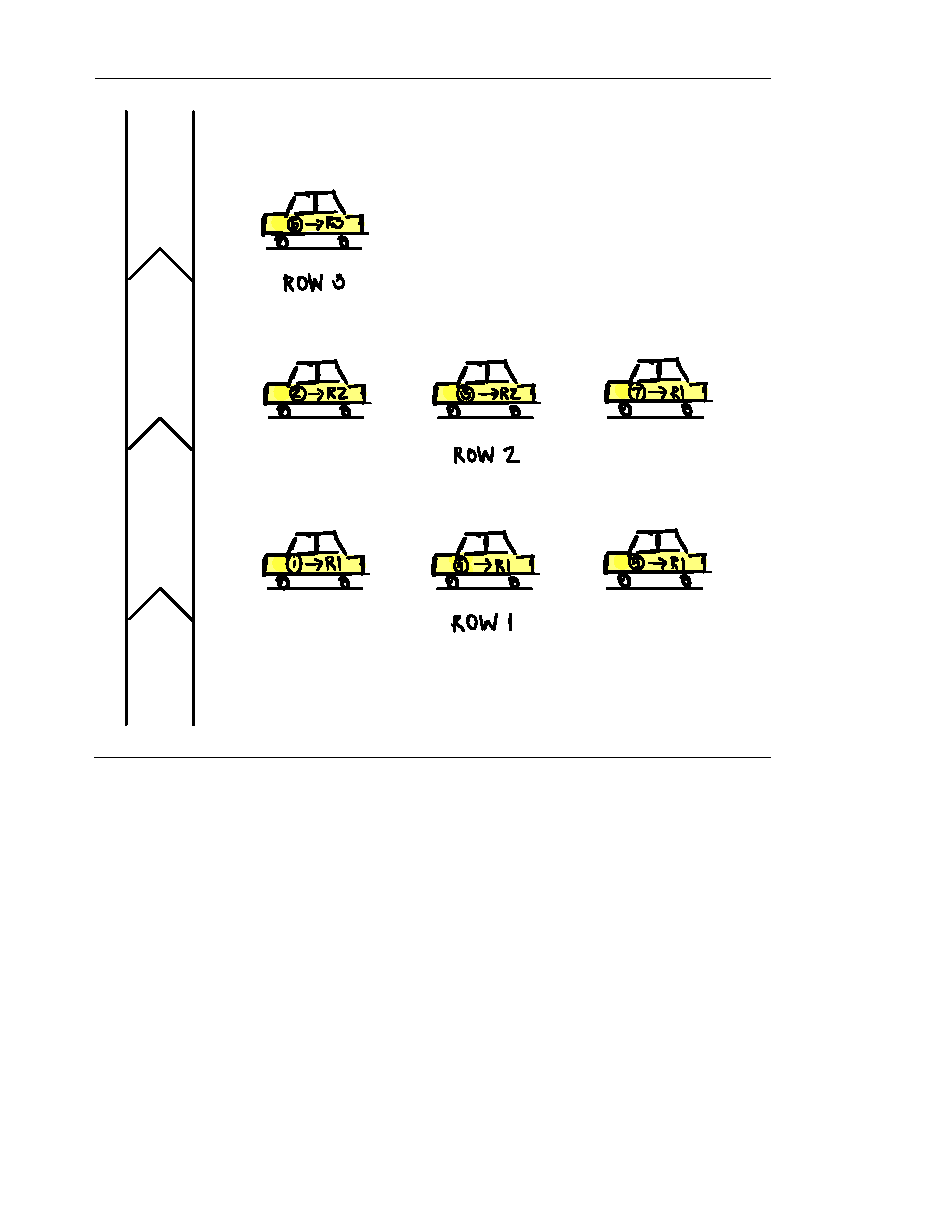
\includegraphics[width = 0.45 \textwidth]{figures/modPFs}
	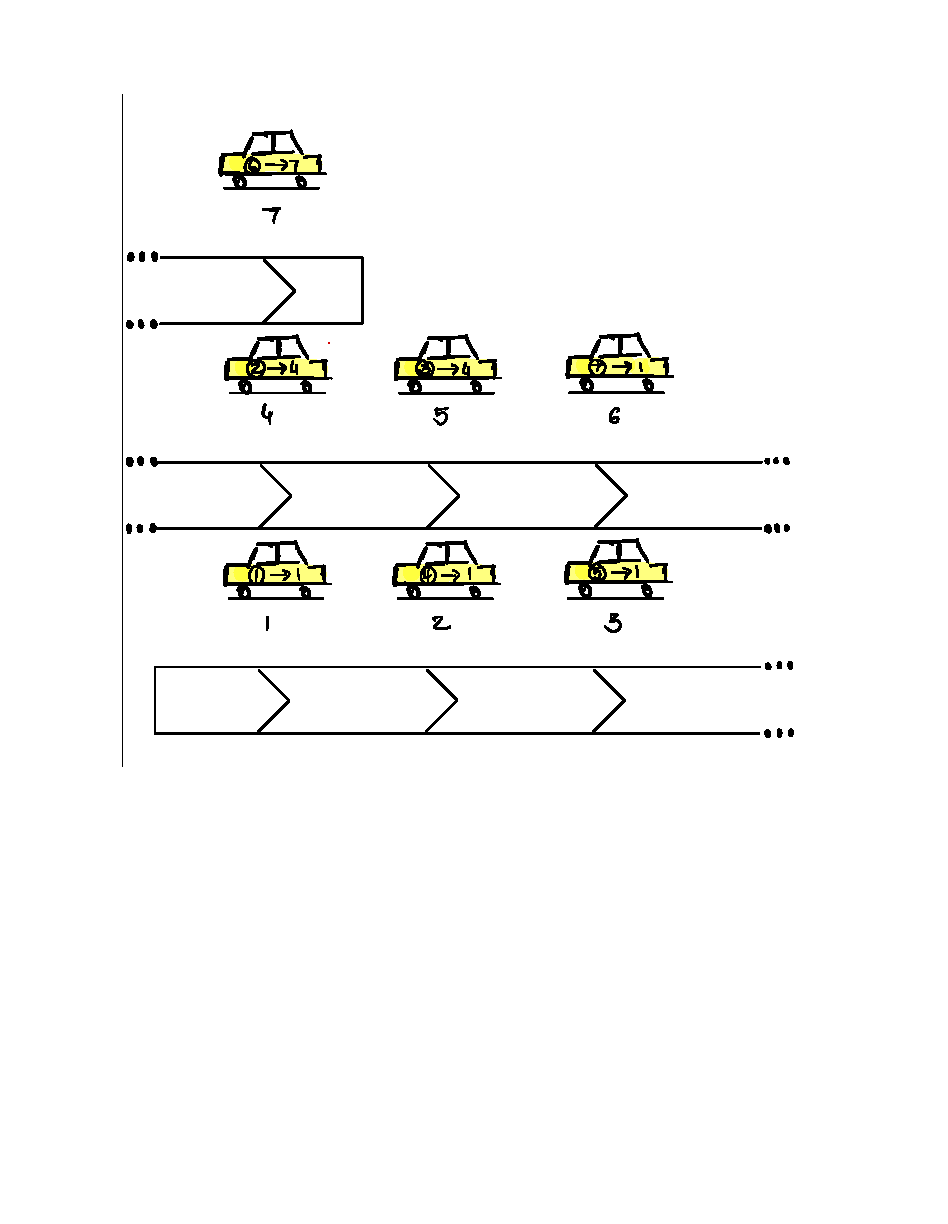
\includegraphics[width = 0.45 \textwidth]{figures/modPFs2}
	\caption{Blake and Konheim's row parking function where cars 1, 4, 5, and 7 prefer the first row, cars 2 and 3 prefer the second row and car 6 prefers the last row can be understood as a restricted parking function $\pi = (1, 4, 4, 1, 1, 7, 1) \in \mathrm{PF}_{7 \mid \{ 1, 4, 7 \}}$. This is an example of the case $g = s = 3$, $k = 2$.}
\end{figure}

\begin{restatable}{theorem}{modPFcount}
	\label{thm:modPFcount}
	The number of parking functions of length $gs - 1$ with gap $g$ between possible preferred spots is
	\[
		\# \mathrm{PF}_{gs - 1 \mid S} = s^{gs - 2}
	\]
	where $S$ is the set of the first $s$ natural numbers $j$ with $j \equiv 1 \pmod g$.
\end{restatable}

This is really the first case of a more general recursive result for parking functions of length $gs - k$. Here compositions $\lambda = (\lambda_{1}, \dots, \lambda_{n})$ with $\sum_{i = 1}^{n} \lambda_{i} = s$ are denoted $\lambda\vDash s, \lvert\lambda\rvert = n$ while $\binom{n}{\lambda}$ denotes the number of ways to partition a set of size $n$ into parts with sizes given by $\lambda_i$.

\begin{restatable}{theorem}{modPFcountGen}
	Given $g,s\in\mathbb{Z}_{>0},$ $1\le k\le gs,$ the number of parking functions of length $gs - k$ with gap $g$ between possible preferred spots is $\mathrm{PF}_{gs - k \mid S \cap [gs - k]}$ and satisfies the relation
	\[
		s^{gs - k} = s \, \# \mathrm{PF}_{gs - k \mid S \cap [gs - k]} + \sum_{n = 2}^{k} \frac{s}{n} \sum_{\lambda \vDash k, \lvert \lambda \rvert = n} \sum_{\mu \vDash s, \lvert \mu \rvert = n} \binom{gs - k}{g \mu - \lambda} \prod_{i = 1}^{n} \# \mathrm{PF}_{g \mu_{i} - \lambda_{i} \mid S \cap [g \mu_{i} - \lambda_{i}]}
	\]
	where $S$ is the set of all natural numbers $j$ with $j \equiv 1 \pmod g$ and $\lambda \vDash k$ indicates that $\lambda$ is a composition of $k$ with length $|\lambda|.$.
\end{restatable}

Note that here, for convenience, $S$ is not a subset of the various $m$ that are the lengths of the parking functions. Rather, $[m] \cap S$ is the relevant subset. 

\begin{proof}
    Consider $gs-k$ cars in a circular parking lot with $gs$ spots; as with the proof above, we only permit cars to prefer the $s$ distinct spots $1,g+1,2g+1,\ldots$ around the lot. There are $s^{gs-k}$ total ways to choose these preferences, and every such choice will lead to all cars parking.

    The $k$ empty spots in the parking lot will be distributed in $n$ contiguous segments for some $1\le n\le k.$ These unfilled segments will all be immediately prior to spots that can be preferred; all other scenarios force cars to pass unfilled spots without parking in them.

    \begin{figure}[H]
    	\centering
	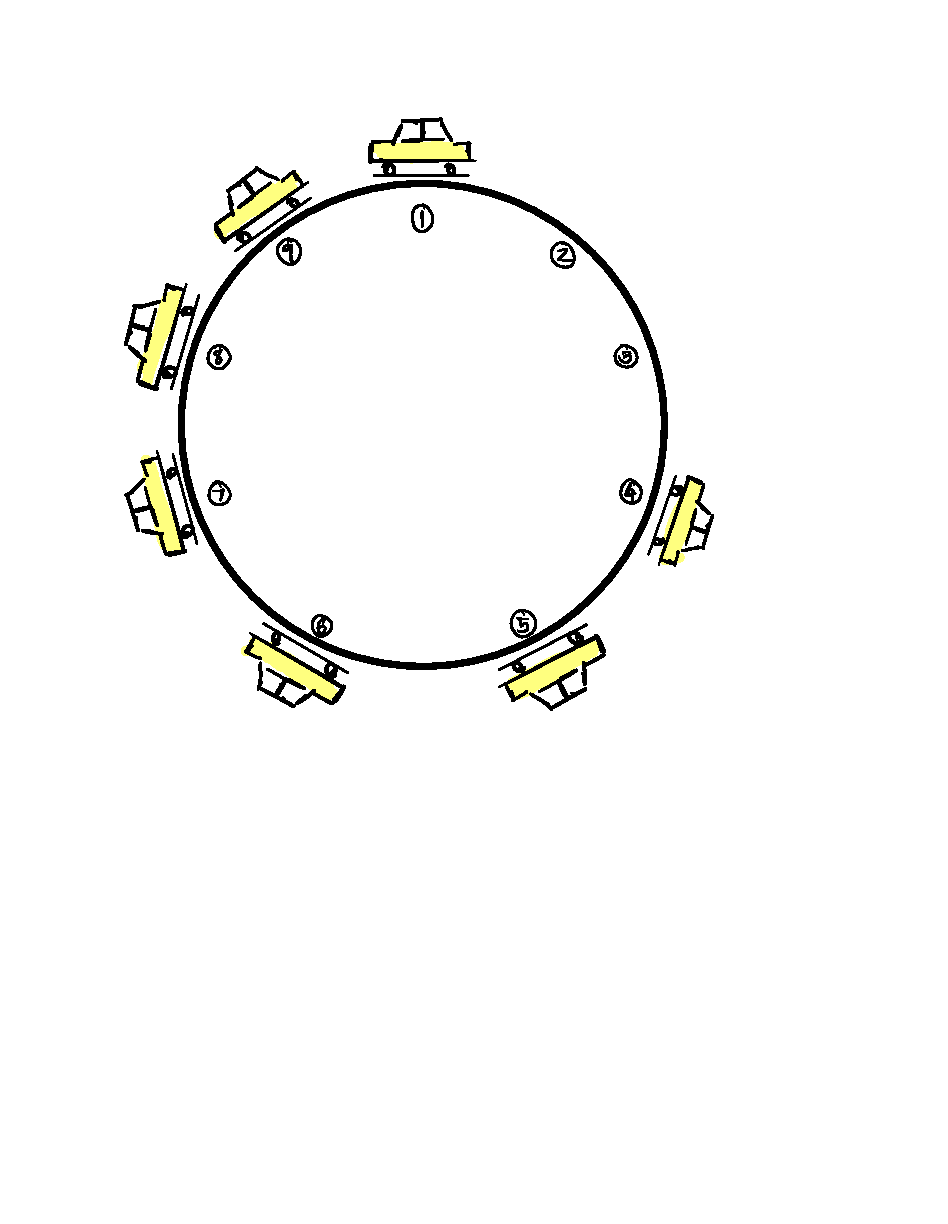
\includegraphics[width = 0.45 \textwidth]{figures/modPFs3}
	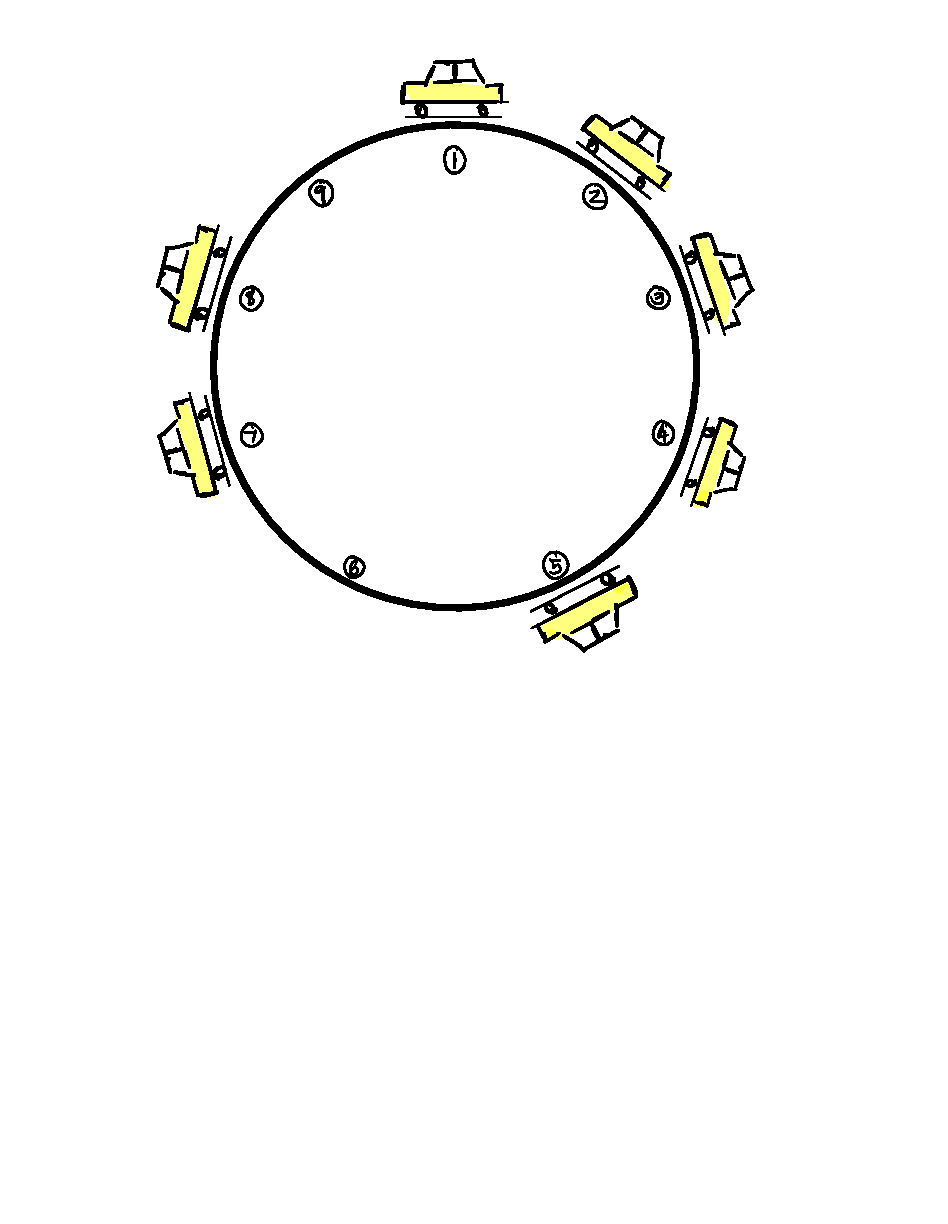
\includegraphics[width = 0.45 \textwidth]{figures/modPFs4}
	\caption{For $g = s = 3$ and $k = 2$, the two empty spots could be the last two spots $g \sigma + 1, g \sigma + 2$ in a ``row'', or the last spots $g \sigma_{1} + 2$ and $g \sigma_{2} + 2$ in two different ``rows''.}
    \end{figure}

    Our gaps will be of size $\lambda_1,\lambda_2,\ldots,\lambda_n,$ all positive and summing up to $k$; we denote this as $\lambda\vDash k,|\lambda|=n.$ These unfilled segments can each be paired with the filled segments immediately prior to them; by virtue of the locations of unfilled segments, these pairs will each have total length a multiple of $g.$ Call these $g\mu_1,g\mu_2,\ldots,g\mu_n$; since the sum of all of these is $gs,$ we have $\mu\vDash s,|\mu|=n.$

    For each such partition of this type, each filled segment will have $g\mu_i-\lambda_i$; choosing which cars will have preferences in each segment can be done in $\binom{gs - k}{g \mu_1 - \lambda_1,g \mu_2 - \lambda_2,\ldots,g \mu_n - \lambda_n}=\binom{gs - k}{g \mu - \lambda}$ ways.
    
    Within each segment, we have $g\mu_i-\lambda_i$ cars which can only prefer spots which are $1$ mod $g$ and must park in the first $g\mu_i-\lambda_i$ spots without gaps. This is precisely a parking function with modular restrictions, and can be done in $\# \mathrm{PF}_{gs - k \mid S \cap [gs - k]}$ ways.

    Finally, we must choose how our parking functions are placed within the circle itself. There are $s$ ways to place the first possible preference in the first restricted parking function, and all placements are forced from there onwards; however, for any given $n$ we are overcounting by a factor of $n,$ since all cyclic permutations of a given $\lambda$ and $\mu$ are equivalent, but all are counted. Thus we multiply by $\frac{s}{n},$ for a total of 
    \[
	    s^{gs - k} = \sum_{n = 1}^{k} \frac{s}{n} \sum_{\lambda \vDash k, \lvert \lambda \rvert = n} \sum_{\mu \vDash s, \lvert \mu \rvert = n} \binom{gs - k}{g \mu - \lambda} \prod_{i = 1}^{n} \# \mathrm{PF}_{g \mu_{i} - \lambda_{i} \mid S \cap [g \mu_{i} - \lambda_{i}]}.
    \]
    The formula above arises from pulling out the desirable $n = 1$ term.
\end{proof}

In practice, the formula it yields is computationally intractable for large $g, s, k$. However, it can be useful to show special cases of small $k$ as in \cref{thm:modPFcount} and below ---

\begin{restatable}{example}{modPFcount2}
	The number of parking functions of length $gs - 2$ cars with gap $g$ between possible preferred spots is
	\[
		\#\mathrm{PF}_{gs - 2 \mid S} = s^{gs - 3} - \frac{1}{2} \sum_{i = 1}^{s - 1} \binom{gs - 2}{gs - 1} i^{gi - 2} (s - i)^{g(s - i) - 2}
	\]
	where $S$ is the set of the first $s$ natural numbers $j$ with $j \equiv 1 \pmod g$.
\end{restatable}

\bibliography{references}
\bibliographystyle{alpha}

\end{document}
